%% ======================================================================
%% 04b_dynamics.tex -- 3. Model (part 2): base, aerial module, and ball dynamics; identification
%% ======================================================================
\subsection{Mobile base dynamics}
\label{sec:basedyn}

\paragraph{Equations of motion}
Applying the Lagrange--d'Alembert principle to the base under constraint \eqref{eq:pfaff} \cite{fierro1997,siciliano2009}, with the center of mass a distance $x_G$ ahead of the axle, yields in $\{B\}$
\begin{align}
  M_{\mathrm{eq}}\,\dot v-M x_G\,\omega^2&=\frac{\tau_R+\tau_L}{r}+M g^{B}_x-C_{rr}Mg\cos\beta\,\operatorname{sign}v, \label{eq:basev}\\
  I_{\mathrm{eq}}\,\dot\omega+M x_G\,v\,\omega&=\frac{b}{2r}(\tau_R-\tau_L)+M x_G\,g^{B}_y-\tau_{\mathrm{scrub}}, \label{eq:basew}
\end{align}
where $M_{\mathrm{eq}}=M+2J_w/r^2$, $I_{\mathrm{eq}}=I_G+Mx_G^2+J_wb^2/(2r^2)$, $J_w$ is the wheel inertia including reflected rotor inertia, $I_G$ is the yaw inertia about the center of mass, $g^{B}_{x,y}$ are the gravity components from \eqref{eq:gB}, and $\tau_{\mathrm{scrub}}$ is the small lateral friction of the omnidirectional wheels. The lateral constraint force at the axle closes the system. Driven by the H-bridge at duty cycle $u_i\in[-1,1]$ with armature inductance neglected, each TorqueNADO motor obeys the averaged torque--speed law
\begin{equation}
  \tau_i=\tau_s\Big(u_i-\frac{\omega_i}{\omega_0}\Big),\qquad \tau_s=\frac{k_tV_b}{R_a}=\SI{4.94}{\newton\metre},\quad \omega_0=\frac{V_b}{k_e}=\SI{10.5}{\radian\per\second},
  \label{eq:motor}
\end{equation}
with datasheet values at the output shaft \cite{pitsco_torquenado}. For straight-line motion at constant speed on a slope $\beta$, \eqref{eq:basev} and \eqref{eq:motor} give the steady-state velocity
\begin{equation}
  v_{ss}(u,\beta)=r\omega_0\Big[u-\frac{rMg(\sin\beta+C_{rr}\cos\beta)}{2\tau_s}\Big].
  \label{eq:vss}
\end{equation}
At the 15\% duty cycle used in the integrated tests and the measured mass ($M=\SI{10.4}{\kilo\gram}$), \eqref{eq:vss} predicts \SI{0.072}{\metre\per\second} on flat ground---matching the 0.06--\SI{0.08}{\metre\per\second} read in LabVIEW telemetry---and \SI{0.027}{\metre\per\second} on the \SI{10}{\degree} ramp. On a \SI{20}{\degree} slope, load torque reaches 18.4\% of stall torque, exceeding the 15\% duty cycle, so the base cannot climb without raising $u$ (Fig.~\ref{fig:base}a). The maximum no-load speed is $r\omega_0=\SI{0.52}{\metre\per\second}$. The initial acceleration from a duty-cycle step $u$ is bounded by $a_0\le 2\tau_su/(Mr)=\SI{2.9}{\metre\per\second\squared}$ for $u=0.15$ (reached when reflected rotor inertia is negligible); this is of the same order as the tip-over limit derived below (and exceeds that of the \SI{10}{\degree} ramp), which is why base references must follow ramps.

\paragraph{Tip-over and traction limits}
Consider the robot climbing a slope $\beta$ with forward acceleration $a$. Taking moments of gravity and d'Alembert forces about the contact line of the driven (rear) wheels, the base does not tip backward as long as
\begin{equation}
  a< a_{\max}(\beta)=g\Big(\frac{x_G}{h_G}\cos\beta-\sin\beta\Big),\qquad\text{i.e.,}\qquad \tan\beta<\frac{x_G}{h_G}\ \ \text{for }a=0 .
  \label{eq:tip}
\end{equation}
Because the octocopter self-levels, its center of mass remains vertically above the spherical joint; repeating the moment balance with its CM at $\vect p_J+h_c\vect z_W$ shows that $h_c$ cancels, so statically the aerial module acts as a point mass at the spherical joint. Static tip-over slopes were measured on 23 November on the complete robot (\SI{10.4}{\kilo\gram}, with all batteries and the module locked) by tilting it manually about each axle to the balance point and reading the angle with an inclinometer: \SI{21.5}{\degree} backward (climbing forward) and \SI{30.5}{\degree} forward (descending forward). With $L=\SI{0.22}{\metre}$, these give $x_G=\SI{88}{\milli\metre}$ and $h_G=\SI{224}{\milli\metre}$. A geometric nuance merits note: when tilting the robot on flat ground about wheels of radius $r=\SI{49.3}{\milli\metre}$, the formula $L/(\tan\theta_A+\tan\theta_B)$ gives the height above the wheel axle ($h_a=\SI{224}{\milli\metre}$, i.e., $h_a+r=\SI{273}{\milli\metre}$ above the ground with the module locked); unlocking the module so it levels on the spherical joint removes the $h_c$ contribution and lowers the effective height by $(m/M)h_c=\SI{44}{\milli\metre}$ to \SI{229}{\milli\metre}. Because these two effects ($+r$ and $-mh_c/M$) nearly cancel, the value $h_G=\SI{224}{\milli\metre}$ used in the leveled-module model differs by only \SI{5}{\milli\metre} (2\%). This confirms the longitudinal CAD position (\SI{81}{\milli\metre}) and rules out an earlier test value (\SI{180}{\milli\metre}). The lateral tip-over angle is $\arctan(b/2h_G)=\SI{40.3}{\degree}$. On the \SI{10}{\degree} ramp, margins of \SI{11.5}{\degree} remain uphill and \SI{20.5}{\degree} downhill. With the module on the spherical joint, the acceleration margin \eqref{eq:tip} is \SI{3.9}{\metre\per\second\squared} on flat ground, \SI{2.1}{\metre\per\second\squared} on the \SI{10}{\degree} ramp, and only \SI{0.26}{\metre\per\second\squared} on a \SI{20}{\degree} slope (Fig.~\ref{fig:base}b). With zero rotor thrust, a \SI{20}{\degree} slope sits at the static stability limit; the course tests are restricted to \SI{10}{\degree}. The friction coefficient required at the driven wheels, $\mu=Mg(\sin\beta+C_{rr}\cos\beta)/N_r$, with rear normal force $N_r=Mg[(L-x_G)\cos\beta+h_G\sin\beta]/L$, is 0.25 at \SI{10}{\degree} and 0.40 at \SI{20}{\degree}---below typical rubber-on-plywood values (0.5--0.8)---so without thrust, traction is not the active limit.

\begin{figure}[!htbp]
  \centering
  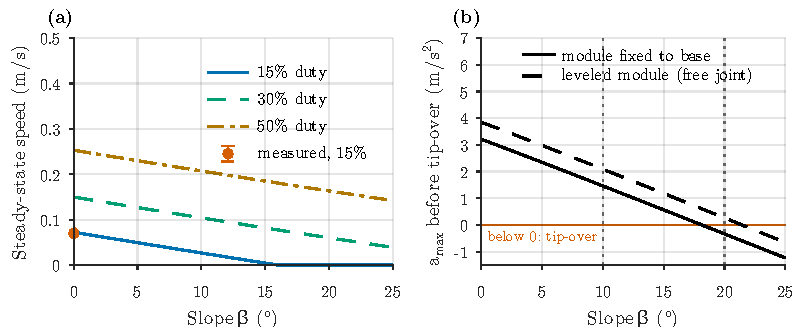
\includegraphics{figures/fig_base_limits.pdf}
  \caption{Mobile base. (a) Steady-state speed versus slope from \eqref{eq:vss} for three duty cycles, together with the measured speed at 15\% on flat ground. (b) Longitudinal acceleration margin before backward tip-over \eqref{eq:tip} with the module on the spherical joint, calibrated against the measured tip-over slope (dot).}
  \label{fig:base}
\end{figure}

\subsection{Aerial module dynamics}
\label{sec:aerial}

\paragraph{Rotor model and control allocation}
Each rotor produces thrust $F_i$ along $\vect z_D$ and reaction torque $-c_Qs_iF_i$ about $\vect z_D$, where $s_i=+1$ for counterclockwise rotors (viewed from above). Using the rotor positions $\vect r_i=[x_i,y_i,h_r]\T$ from Table~\ref{tab:params}, the collective thrust and body-frame torques are
\begin{equation}
  \begin{bmatrix}T\\ \tau_x\\ \tau_y\\ \tau_z\end{bmatrix}=\underbrace{\begin{bmatrix}\vect 1\T\\ \vect y\T\\ -\vect x\T\\ -c_Q\vect s\T\end{bmatrix}}_{\vect B\in\mathbb R^{4\times8}}\vect F,
  \qquad \vect B\vect B\T=\diag\big(8,\ 4L_r^2,\ 4L_r^2,\ 8c_Q^2\big),
  \label{eq:alloc}
\end{equation}
because $\sum x_i=\sum y_i=\sum s_i=\sum x_iy_i=\sum s_ix_i=\sum s_iy_i=0$ and $\sum x_i^2=\sum y_i^2=4L_r^2$ for the octocopter geometry (arm height $h_r$ does not contribute because thrust is parallel to $\vect z_D$). The four channels are therefore orthogonal, and the minimum-norm allocation is explicit:
\begin{equation}
  \vect F=\vect B\T(\vect B\vect B\T)^{-1}\vect w=\frac{T}{8}\vect 1+\frac{\vect y\,\tau_x-\vect x\,\tau_y}{4L_r^2}-\frac{\vect s\,\tau_z}{8c_Q},\qquad \vect w=[T,\tau_x,\tau_y,\tau_z]\T .
  \label{eq:alloc_inv}
\end{equation}
The firmware implements \eqref{eq:alloc_inv} directly \cite{johansen2013}: the collective sets the baseline force $F_0=T/8$, roll and pitch increments are added, and the yaw increment is added along the yaw row projected onto the null space of the other three rows (which, by the orthogonality above, is the yaw row itself). When an increment would drive any rotor outside $[F_{\min},F_{\max}]$ (\SIrange{1180}{2000}{\micro\second}), roll and pitch are scaled first and yaw second. For pure pitch torque, the $x$-axis rotors ($|x_i|=L_r$) saturate first, giving the achievable torque
\begin{equation}
  |\tau_y|_{\max}=4L_r\,\min\{F_{\max}-F_0,\ F_0-F_{\min}\},
  \label{eq:taumax}
\end{equation}
which, under the firmware thrust map, equals \SI{3.2}{\newton\metre} at a collective of \SI{1750}{\micro\second} and \SI{2.4}{\newton\metre} at \SI{1816}{\micro\second}---well above the torques required in hover (Section~\ref{sec:authority}). The firmware converts each force to a pulse width by inverting $F=k_F\big((u-u_0)/\SI{860}{\micro\second}\big)^n$ with $k_F=\SI{5.40}{\newton}$; if the true gain is $k_F'$, every torque generated by the controller is multiplied by the thrust-gain ratio $k_T=k_F'/k_F$, identified in Section~\ref{sec:ident}.

\paragraph{Newton--Euler equations about the moving pivot}
The rotating assembly (mass $m$, inertia $\vect J$ about the spherical joint, center of mass at $\vect r_c=[\delta_x,\delta_y,h_c]\T$ in $\{D\}$) rotates about the spherical joint center, a body-fixed point whose acceleration $\vect a_J$ \eqref{eq:aJ} is imposed by the base and vertical guide. For a body-fixed point on a rigid body, the angular momentum about it is $\vect J\vect\omega_D$, and its inertial derivative equals the external moment minus $m\,\vect r_c\times\vect a_J$ \cite{ginsberg1998}. In $\{D\}$ components:
\begin{equation}
  \vect J\dot{\vect\omega}_D+\vect\omega_D\times\vect J\vect\omega_D=
  \underbrace{\sum_{i=1}^{8}\vect r_i\times F_i\ez-\sum_{i=1}^{8}c_Qs_iF_i\ez}_{[\tau_x,\ \tau_y,\ \tau_z]\T}
  +\,m\,\vect r_c\times\Rot_{WD}\T\big(\vect g_W-\vect a_J\big)-\vect\tau_f ,
  \label{eq:euler}
\end{equation}
with $\vect g_W=[0,0,-g]\T$ and spherical-joint friction $\vect\tau_f$. The third term contains the three couplings that dominate module behavior. Linearizing about level hover (verified symbolically, \ref{app:derivations}):
\begin{align}
  J_x\ddot\phi&=\tau_x+m(g+a_{J,z})h_c\,\phi+m h_c\,a_{J,y}-m g\,\delta_y, \label{eq:rolllin}\\
  J_y\ddot\theta&=\tau_y+m(g+a_{J,z})h_c\,\theta-m h_c\,a_{J,x}+m g\,\delta_x, \label{eq:pitchlin}
\end{align}
with $\vect a_J$ in $\{D\}$ components. (i) Because $h_c>0$, the module is an inverted pendulum on the spherical joint, with open-loop poles $\pm p$, $p=\sqrt{mgh_c/J_y}=\SI{6.1}{\radian\per\second}$ for $h_c=\SI{0.14}{\metre}$ (doubling time \SI{0.11}{\second}). (ii) Horizontal base acceleration produces the torque $\mp mh_ca_J$: the top of the module lags behind the spherical joint, which is the primary disturbance path from the base to the octocopter. (iii) A horizontal CM eccentricity $\delta$ produces a constant torque $mg\delta$ that the controller must permanently oppose. Vertical spherical-joint acceleration parametrically modulates pendulum stiffness.

Along the vertical guide (axis $\vect z_B$), the carriage and module obey
\begin{equation}
  (m+m_c)\ddot d=T\,\vect z_D\!\cdot\!\vect z_B-(m+m_c)\big(g\cos\beta+\vect a_B\!\cdot\!\vect z_B\big)-F_g(\dot d)+F_{\mathrm{stop}},
  \label{eq:guide}
\end{equation}
so the module lifts off when $T>(m+m_c)g\cos\beta+F_{g,\mathrm{static}}$. While $T$ stays lower, the module rests on the lower stop and transmits its weight minus $T$ to the base; this is the weight relief exploited on the ramp (Section~\ref{sec:porquedron}).

\paragraph{Hover power}
By momentum theory \cite{leishman2006}, hover thrust per rotor, $T/8=\SI{4.41}{\newton}$, across a 9.4-inch propeller disk induces a velocity $v_h=\sqrt{T/(16\rho A)}=\SI{6.4}{\metre\per\second}$ and requires an ideal power of $Tv_h/8=\SI{28}{\watt}$ per rotor. With a figure of merit of 0.5 and a motor--ESC efficiency of 0.8, the eight rotors draw roughly \SI{570}{\watt}; the A2212 datasheet table with a 9450 propeller, scaled to \SI{3.6}{\kilo\gram}, gives \SI{500}{\watt}. That equals 22--\SI{25}{\ampere} per fused branch, and power grows as $T^{3/2}$, so every collective increase to offset voltage sag costs current. This is why the firmware limits operation above \SI{1850}{\micro\second} to \SI{20}{\second} (\SI{30}{\ampere} fuses), and why a \SI{29}{\milli\metre} propeller tip clearance was kept with $L_r=\SI{0.350}{\metre}$. Section~\ref{sec:bateria} translates these figures into thrust margin and endurance.

\subsection{Aerial module identification from hover telemetry}
\label{sec:ident}

\paragraph{Thrust gain}
At liftoff, \eqref{eq:guide} gives $8k_F'\big((u-u_0)/860\big)^n=(m+m_c)g+F_{g,\mathrm{static}}$. Liftoff occurred between \SI{1725}{\micro\second} and \SI{1775}{\micro\second} with charged LiPo packs at 12.4\,V at rest at the start of the session (Section~\ref{sec:flights}); neglecting guide friction yields lower bounds $k_F'=$ \SIrange{7.17}{8.18}{\newton}, so the thrust-gain ratio is $k_T=1.33$--1.52 (Fig.~\ref{fig:ident}b). The firmware map, and the Isaac Lab model built on it, predicted hover at \SI{1899}{\micro\second}; an independent power audit based on motor and propeller data predicted \SI{1770}{\micro\second}, inside the measured band, though for a mass of \SI{3.10}{\kilo\gram} rather than \SI{3.6}{\kilo\gram}.

\paragraph{Center of mass}
During quasi-static hover ($\dot{\vect\omega}_D\approx\vect 0$, integrators settled, $T\approx(m+m_c)g$), \eqref{eq:rolllin}--\eqref{eq:pitchlin} reduce to moment balances. Dividing by collective thrust cancels the unknown gain $k_F'$ and leaves the center-of-thrust coordinates,
\begin{equation}
  x_{cp}=\frac{\sum_i x_iF_i}{\sum_iF_i}=c\,(\delta_x+h_c\sin\theta),\qquad
  y_{cp}=\frac{\sum_i y_iF_i}{\sum_iF_i}=c\,(\delta_y-h_c\sin\phi),
  \label{eq:cop}
\end{equation}
with $c=m/(m+m_c)$, which is linear in $(\delta_x,\delta_y,h_c)$ and computed from logged motor commands. Averaging \eqref{eq:cop} over the hover phase of the seven flights that lifted off (samples with $|p|,|q|<\SI{15}{\degree\per\second}$ above \SI{1650}{\micro\second}) and solving the 14 equations by least squares gives
\begin{equation}
  \hat\delta_x=9.5\pm1.8\ \mathrm{mm},\qquad \hat\delta_y=1.9\pm1.5\ \mathrm{mm},\qquad \hat h_c=0.14\pm0.06\ \mathrm{m}\quad(\pm1\sigma),
  \label{eq:idres}
\end{equation}
with an RMS residual of \SI{3.3}{\milli\metre} (Fig.~\ref{fig:ident}a). The estimate of $h_c$ shifts by less than its uncertainty when the map exponent varies between 1.3 and 1.6 (0.11--\SI{0.14}{\metre}), and agrees with the \SI{0.10}{\metre} value from the CAD model. The eccentricity produces a constant gravity torque $mg\delta_x=\SI{0.31}{\newton\metre}$ toward M8.

\begin{figure}[!htbp]
  \centering
  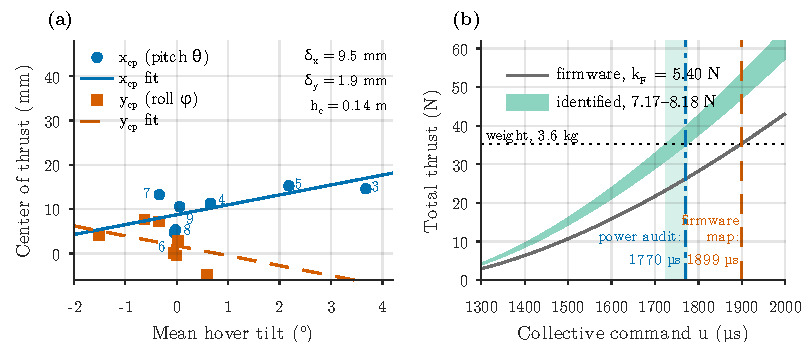
\includegraphics{figures/fig_ident.pdf}
  \caption{Identification from hover telemetry. (a) Center of thrust versus mean tilt across the seven hover flights (labels: flight number) and least-squares fit of \eqref{eq:cop}. (b) Total thrust from the firmware map, band identified from the liftoff condition, moving-assembly weight, and hover predictions from the firmware map and power audit.}
  \label{fig:ident}
\end{figure}

\subsection{Ball on an accelerating and rotating plate}
\label{sec:ball}

Let $\vect\Omega$ be the angular velocity of the plate frame $\{P\}$ and let $\vect a_G$ be the absolute acceleration of its origin (the universal joint center), both expressed in $\{P\}$. The ball center is at $\vect\rho=[x_b,y_b,\varepsilon]\T$, its absolute angular velocity is $\vect\omega_b$, and rolling without slip (A6) requires the contact-point velocity of the ball to equal that of the plate surface beneath it. This gives $\dot{\vect\rho}=r_b(\vect\omega_b-\vect\Omega)\times\ez$, i.e., the relative angular velocity is $\vect w=\vect\omega_b-\vect\Omega=[-\dot y_b/r_b,\ \dot x_b/r_b,\ w_z]\T$, with a free spin $w_z$ about the plate normal. Writing Newton's law for the ball center in the rotating frame and Euler's law for the ball about its center, with the contact force applied at $-r_b\ez$, and eliminating the tangential contact forces (\ref{app:derivations}) yields, exactly,
\begin{align}
  \frac{\ddot x_b}{\gamma_b}&=g_x-a_{G,x}-\kappa\dot\Omega_y+\dot\Omega_z\,y_b+(\Omega_y^2+\Omega_z^2)\,x_b-\Omega_x\Omega_y\,y_b \notag\\
   &\quad-\varepsilon\,\Omega_x\Omega_z+(2+\iota)\,\Omega_z\dot y_b+\iota r_b\,\Omega_xw_z, \label{eq:ballx}\\
  \frac{\ddot y_b}{\gamma_b}&=g_y-a_{G,y}+\kappa\dot\Omega_x-\dot\Omega_z\,x_b+(\Omega_x^2+\Omega_z^2)\,y_b-\Omega_x\Omega_y\,x_b \notag\\
   &\quad-\varepsilon\,\Omega_y\Omega_z-(2+\iota)\,\Omega_z\dot x_b+\iota r_b\,\Omega_yw_z, \label{eq:bally}\\
  \dot w_z&=-\dot\Omega_z-\frac{\Omega_x\dot x_b+\Omega_y\dot y_b}{r_b}, \label{eq:spin}
\end{align}
where $[g_x,g_y,g_z]\T=\Rot_{WP}\T\vect g_W$ is gravity in $\{P\}$, $\iota=I_b/(m_br_b^2)$ ($2/5$ for a solid sphere), $\gamma_b=1/(1+\iota)$, and
\begin{equation}
  \kappa=\varepsilon+\frac{I_b}{m_br_b}=\varepsilon+\iota r_b=\SI{42.3}{\milli\metre}
  \label{eq:kappa}
\end{equation}
is the effective height of the ball above the rotation axis. Equations \eqref{eq:ballx}--\eqref{eq:spin} contain the classical ball-and-plate model as the special case $\vect a_G=\vect 0$, $\Omega_z=0$, $\varepsilon=0$ \cite{awtar2002,hauser1992}; the additional terms are the translational acceleration of the plate center, the Euler term $\kappa\dot{\vect\Omega}$ from ball height, centrifugal and Coriolis terms from base rotation, and spin coupling.

\paragraph{Linearization and transfer functions}
For small angles, $g_x\simeq g\,\Theta_P$ and $g_y\simeq-g\,\Phi_P$; with \eqref{eq:tilt} and the linearization of \eqref{eq:aG}, $a_{G,x}\simeq a_{J,x}+h_P\ddot\theta$ and $a_{G,y}\simeq a_{J,y}-h_P\ddot\phi$, the ball obeys
\begin{align}
  \ddot x_b&=\gamma_b\Big[g(\theta+\alpha_y)-\kappa\,\ddot\alpha_y-(h_P+\kappa)\,\ddot\theta-a_{J,x}\Big], \label{eq:balllinx}\\
  \ddot y_b&=\gamma_b\Big[-g(\phi+\alpha_x)+\kappa\,\ddot\alpha_x+(h_P+\kappa)\,\ddot\phi-a_{J,y}\Big]. \label{eq:balllinly}
\end{align}
Equations \eqref{eq:balllinx}--\eqref{eq:balllinly} summarize the coupling across the entire robot: the ball is driven by servo tilt (the control input), residual octocopter attitude amplified by the lever arm $h_P+\kappa=\SI{0.146}{\metre}$, and spherical-joint acceleration produced by the base. With $\alpha_y=K_\alpha u$, the three $x$-axis transfer functions are
\begin{equation}
  \frac{X_b}{U}=K_b\,\frac{1-s^2/z_1^2}{s^2},\qquad
  \frac{X_b}{\Theta}=\gamma_b g\,\frac{1-s^2/z_2^2}{s^2},\qquad
  \frac{X_b}{A_{J,x}}=-\frac{\gamma_b}{s^2},
  \label{eq:balltf}
\end{equation}
with plant gain $K_b=\gamma_bgK_\alpha=\SI{6.0}{\milli\metre\per\second\squared}$ per microsecond (solid sphere) and zeros $z_1=\sqrt{g/\kappa}=\SI{15.2}{\radian\per\second}$ and $z_2=\sqrt{g/(h_P+\kappa)}=\SI{8.2}{\radian\per\second}$. Each pair contains a right-half-plane zero: the servo path is non-minimum phase (a rapid tilt initially pushes the ball in the wrong direction because the plate surface accelerates beneath it), and above $z_2/2\pi=\SI{1.3}{\hertz}$ octocopter angular acceleration disturbs the ball more than its tilt.

\paragraph{Base rotation}
For a base turning at constant rate $\omega$ ($\vect\Omega=\omega\ez$), \eqref{eq:ballx}--\eqref{eq:bally} add negative stiffness $\gamma_b\omega^2$ and gyroscopic coupling $\gamma_b(2+\iota)\omega$ between axes. Even for a turn faster than any test ($\omega=\SI{0.53}{\radian\per\second}$, wheels at $\pm\SI{0.10}{\metre\per\second}$), the negative stiffness is \SI{0.20}{\per\second\squared}, less than 10\% of the stiffness $K_bk_p\approx\SI{2}{\per\second\squared}$ provided by the ball controller (Section~\ref{sec:ballcontrol}).
